% 
% LaTeX Problem Set Template by Sachin Padmanabhan
% I created this when I was a freshman in CS 103,
% and I continue to use it to this day.
%
% Hope you enjoy!
%
% There may be problems with this template.
% If so, feel free to contact me.
%

\documentclass{article}
\usepackage{amsmath}
\usepackage{amssymb}
\usepackage{amsthm}
\usepackage{amssymb}
\usepackage{mathdots}
\usepackage[pdftex]{graphicx}
\usepackage{fancyhdr}
\usepackage[margin=1in]{geometry}
\usepackage{multicol}
\usepackage{bm}
\usepackage{listings}
\PassOptionsToPackage{usenames,dvipsnames}{color}  %% Allow color names
\usepackage{pdfpages}
\usepackage{algpseudocode}
\usepackage{tikz}
\usepackage{enumitem}
\usepackage[T1]{fontenc}
\usepackage{inconsolata}
\usepackage{framed}
\usepackage{wasysym}
\usepackage[thinlines]{easytable}
\usepackage{hyperref}
\hypersetup{
    colorlinks=true,
    linkcolor=blue,
    filecolor=magenta,      
    urlcolor=blue,
}

\title{CS 103: Mathematical Foundations of Computing\\Problem Set \#1}
\author{Sachin Padmanabhan}
\date{\today}

\lhead{Sachin Padmanabhan}
\chead{Problem Set \#1}
\rhead{\today}
\lfoot{}
\cfoot{CS 103: Mathematical Foundations of Computing --- Winter 2017}
\rfoot{\thepage}

\newcommand{\abs}[1]{\lvert #1 \rvert}
\newcommand{\absfit}[1]{\left\lvert #1 \right\rvert}
\newcommand{\norm}[1]{\left\lVert #1 \right\rVert}
\newcommand{\eval}[3]{\left[#1\right]_{#2}^{#3}}
\renewcommand{\(}{\left(}
\renewcommand{\)}{\right)}
\newcommand{\floor}[1]{\left\lfloor#1\right\rfloor}
\newcommand{\ceil}[1]{\left\lceil#1\right\rceil}
\newcommand{\pd}[1]{\frac{\partial}{\partial #1}}
\newcommand{\inner}[1]{\langle#1\rangle}
\newcommand{\cond}{\bigg|}
\newcommand{\rank}[1]{\mathbf{rank}(#1)}
\newcommand{\range}[1]{\mathbf{range}(#1)}
\newcommand{\nullsp}[1]{\mathbf{null}(#1)}
\newcommand{\repr}[1]{\left\langle#1\right\rangle}

\DeclareMathOperator{\Var}{Var}
\DeclareMathOperator{\tr}{tr}
\DeclareMathOperator{\Tr}{\mathbf{Tr}}
\DeclareMathOperator{\diag}{\mathbf{diag}}
\DeclareMathOperator{\dist}{\mathbf{dist}}
\DeclareMathOperator{\prob}{\mathbf{prob}}
\DeclareMathOperator{\dom}{\mathbf{dom}}
\DeclareMathOperator{\E}{\mathbf{E}}
\DeclareMathOperator{\R}{\mathbb{R}}
\DeclareMathOperator{\var}{\mathbf{var}}
\DeclareMathOperator{\quartile}{\mathbf{quartile}}
\DeclareMathOperator{\conv}{\mathbf{conv}}
\DeclareMathOperator{\VC}{VC}
\DeclareMathOperator*{\argmax}{arg\,max}
\DeclareMathOperator*{\argmin}{arg\,min}
\DeclareMathOperator{\Ber}{Bernoulli}
\DeclareMathOperator{\NP}{\mathbf{NP}}
\DeclareMathOperator{\coNP}{\mathbf{coNP}}
\DeclareMathOperator{\TIME}{\mathsf{TIME}}
\DeclareMathOperator{\polytime}{\mathbf{P}}
\DeclareMathOperator{\PH}{\mathbf{PH}}
\DeclareMathOperator{\SIZE}{\mathbf{SIZE}}
\DeclareMathOperator{\ATIME}{\mathbf{ATIME}}
\DeclareMathOperator{\SPACE}{\mathbf{SPACE}}
\DeclareMathOperator{\ASPACE}{\mathbf{ASPACE}}
\DeclareMathOperator{\NSPACE}{\mathbf{NSPACE}}
\DeclareMathOperator{\Z}{\mathbb{Z}}
\DeclareMathOperator{\N}{\mathbb{N}}
\DeclareMathOperator{\EXP}{\mathbf{EXP}}
\DeclareMathOperator{\NEXP}{\mathbf{NEXP}}
\DeclareMathOperator{\NTIME}{\mathbf{NTIME}}
\DeclareMathOperator{\DTIME}{\mathbf{DTIME}}
\DeclareMathOperator{\poly}{poly}
\DeclareMathOperator{\BPP}{\mathbf{BPP}}
\DeclareMathOperator{\ZPP}{\mathbf{ZPP}}
\DeclareMathOperator{\RP}{\mathbf{RP}}
\DeclareMathOperator{\coRP}{\mathbf{coRP}}
\DeclareMathOperator{\BPL}{\mathbf{BPL}}
\DeclareMathOperator{\IP}{\mathbf{IP}}
\DeclareMathOperator{\PSPACE}{\mathbf{PSPACE}}
\DeclareMathOperator{\NPSPACE}{\mathbf{NPSPACE}}
\DeclareMathOperator{\SAT}{\mathsf{SAT}}
\DeclareMathOperator{\NL}{\mathbf{NL}}
\DeclareMathOperator{\PCP}{\mathbf{PCP}}
\DeclareMathOperator{\PP}{\mathbf{PP}}
\DeclareMathOperator{\cost}{cost}
\let\Pr\relax
\DeclareMathOperator*{\Pr}{\mathbf{Pr}}

\definecolor{shadecolor}{gray}{0.95}

\theoremstyle{plain}
\newtheorem*{lem}{Lemma}

\theoremstyle{plain}
\newtheorem*{claim}{Claim}

\theoremstyle{definition}
\newtheorem*{answer}{Answer}

\newtheorem{theorem}{Theorem}[section]
\newtheorem*{thm}{Theorem}
\newtheorem{corollary}{Corollary}[theorem]
\newtheorem{lemma}[theorem]{Lemma}

\renewcommand{\headrulewidth}{0.4pt}
\renewcommand{\footrulewidth}{0.4pt}

\setlength{\parindent}{0pt}

\pagestyle{fancy}

\renewcommand{\thefootnote}{\fnsymbol{footnote}}

\begin{document}

\maketitle

\section{Set Theory Warmup}

This question is designed to help you get used to the notation and mathematical
conventions surrounding sets.
Consider the following sets:
\begin{align*}
A &= \{1, 2, 3, 4\} \\
B &= \{2, 2, 2, 1, 4, 3\} \\
C &= \{1, \{2\}, \{\{3, 4\}\}\} \\
D &= \{1, 3\} \\
E &= \N \\
F &= \{\N\}
\end{align*}
Answer each of the following questions and briefly justify your answers.
No proofs are necessary.

\begin{enumerate}[label*=\roman*.,ref=\roman*]

\item Which pairs of the above sets, if any, are equal to one another?

\begin{shaded}
\begin{answer}
Write your answer here.
\end{answer}
\end{shaded}

\item Is $D \in A$? Is $D \subseteq A$?

\begin{shaded}
\begin{answer}
Write your answer here.
\end{answer}
\end{shaded}

\item What is $A \cap C$? How about $A \cup C$? How about $A \Delta C$?

\begin{shaded}
\begin{answer}
Write your answer here.
\end{answer}
\end{shaded}

\item What is $A - C$? How about $\{A - C\}$? Are those sets equal?

\begin{shaded}
\begin{answer}
Write your answer here.
\end{answer}
\end{shaded}

\item What is $|B|$? What is $|E|$? What is $|F|$?

\begin{shaded}
\begin{answer}
Write your answer here.
\end{answer}
\end{shaded}

\item What is $E - A$? Express your answer in set-builder notation.

\begin{shaded}
\begin{answer}
Write your answer here.
\end{answer}
\end{shaded}

\item Is $0 \in E$? Is $0 \in F$?

\begin{shaded}
\begin{answer}
Write your answer here.
\end{answer}
\end{shaded}

\end{enumerate}

\section{The Power Set Revisited}

In our first lecture, we saw an operation called the power set that, given a set $S$, produces a set $\wp(S)$ consisting of all the subsets of the set $S$. Why \textit{didn't} we introduce an operation that, given a set $S$, produces a set consisting of all the \textit{elements} of $S$?

\begin{shaded}
\begin{answer}
Write your answer here.
\end{answer}
\end{shaded}

\section{Much Ado About Nothing}

\begin{shaded}
Submit your six $\mathsf{.object}$ files through GradeScope.
\end{shaded}

\section{Set Theory in C++}

\begin{shaded}
Submit your edited $\mathsf{SetTheory.cpp}$ file through GradeScope.
\end{shaded}

\section{Describing the World in Set Theory}

The notation of set theory (e.g. $\cup, \cap, \wp, \subseteq, \in$, etc.) is a great tool for describing the real world. Answer
each of the following questions by writing an expression using set theory notation, but \textit{\textbf{without}} using
plain English, \textit{\textbf{without}} using set-builder notation, \textit{\textbf{without}} introducing any new variables, and without using propositional or first-order logic (which we'll cover next week).

\begin{enumerate}[label*=\roman*.,ref=\roman*]

\item Let's have $C$ be the set of US citizens, $S$ the set of people who live in a US state, $M$ be the set of
all people eighteen and older, and $V$ be the set of people who are allowed to vote in US presidential
elections. Write an expression that says that every US citizen age eighteen and older who
lives in a US state can vote in a US presidential election.

\textit{\textcolor{blue}{Once you've written up your answer to this problem, take a minute to \textbf{type-check} it. As an example, suppose
that you have the following answer: 
\begin{equation*}
(C \in M) \cap (V \in M)
\end{equation*}
This expression can't possibly be right, and here's one way to see this. The expression $C \in M$ is of type
boolean -- either $C \in M$ is true or it isn't -- and the same is true of $V \in M$. However, the intersection operator
$\cap$ can only be applied to sets. The expression therefore contains a type error: it tries to apply an operator that only works on sets to boolean values. }}

\begin{shaded}
\begin{answer}
Write your answer here.
\end{answer}
\end{shaded}

\item Suppose you're on an exciting first date. Let $Y$ represent your hobbies and $D$ represent your
date's hobbies. Write an expression that says that you have a hobby that your date doesn't have.

\textit{\textcolor{blue}{You can type-check this answer in a different way. For example, suppose you came up with this expression:
\begin{equation*}
Y \cup D
\end{equation*}
Here, $Y$ and $D$ are sets, so it's perfectly fine to write $Y \cup D$, which evaluates to an object of type set. But
notice that the statement here asks you to write an expression that says ``you have a hobby that your date
doesn't have,'' and that statement is essentially of type boolean (you either do or do not have a hobby your
date doesn't have). Therefore. $Y \cup D$ can't possibly be an expression with the right meaning, since the type
of the expression (set) doesn't match the type of the statement (boolean). }}

\begin{shaded}
\begin{answer}
Write your answer here.
\end{answer}
\end{shaded}

\item Tom Stoppard's play \textit{Rosencrantz and Guildenstern are Dead} contains this quote in which the
leader of a theater troupe discusses what sorts of plays his group is willing to put on:
\begin{quote}
``We're more of the love, blood, and rhetoric school. Well, we can do you blood and
love without the rhetoric, and we can do you blood and rhetoric without the love,
and we can do you all three concurrent or consecutive. But we can't give you love
and rhetoric without the blood. Blood is compulsory.''
\end{quote}
Let $B$ be the set of all plays involving blood, $L$ be the set of all plays involving love, and $R$ be the
set of all plays involving rhetoric. Write an expression for all plays involving at least one of
blood, love, and rhetoric which also happen to include blood.

\begin{shaded}
\begin{answer}
Write your answer here.
\end{answer}
\end{shaded}

\item In the Talking Heads song \textit{Crosseyed and Painless}, David Byrne speaks the following lines:
\begin{center}
``Facts are simple and facts are straight. \\
Facts are lazy and facts are late.''
\end{center}
Let $F$ be the set of all facts. Let $A, B, C,\text{ and }D$ represent the set of all things that are simple,
straight, lazy, and late, respectively. Write an expression that conveys David Byrne's lyrics in the
language of set theory.

\begin{shaded}
\begin{answer}
Write your answer here.
\end{answer}
\end{shaded}

\item Let's say that a \textit{\textbf{committee}} is a group of people, which we can think of as being represented by
the set of people on that committee. Let's have $S$ represent the set of all students at Stanford and
let $F$ represent the set of all faculty at Stanford. Write an expression representing the set of all
committees you can make from Stanford students and faculty that contain at least one student
and at least one faculty member. You can assume no one is both a student and a faculty member.

\textit{\textcolor{blue}{Something to think about: how would you say ``all committees made purely of students?'' }}

\begin{shaded}
\begin{answer}
Write your answer here.
\end{answer}
\end{shaded}

\end{enumerate}

\section{Modular Arithmetic}

Different numbers can yield the same remainder when divided by some number.
For example,
the numbers $1$, $12$, $23$, and $34$ all leave a remainder of one
when divided by eleven.
To formalize this relationship between numbers,
we'll introduce a relation $\equiv_k$ that, intuitively,
indicates that two numbers leave the same remainder when divided by $k$.
For example,
we'd say that $1 \equiv_{11} 12$, since both 1 and 12 leave a
remainder of 1 when divided by 11, and that $8\equiv_3 14$, 
since both 8 and 14 leave a remainder of 2 when
divided by 3. To be more rigorous, we'll formally define $\equiv_k$.
For any integer $k$,
define $a \equiv_k b$ as follows:
\begin{center}
We say that $a \equiv_k b$ if there exists an integer $q$ such that
$a - b = kq$.
\end{center}
For example, $7 \equiv_3 4$ because $7 - 4 = 3 = 3 \cdot 1$,
and $13 \equiv_4 5$ because $13 - 5 = 8 = 4 \cdot 2$.
If $x \equiv_k y$,
we say that \textit{\textbf{x is congruent to y modulo k}},
hence the terminology in the checkpoint problem.
In this problem, you will prove several properties of modular congruence.

\begin{enumerate}[label*=\roman*.,ref=\roman*]

\item Prove that for any integer $x$ and any integer $k$
that $x \equiv_k x$.

\textit{\textcolor{blue}{ Be careful not to assume what you need to prove. Don't start your proof by assuming that there's a choice of $q$ where $x - x = kq$ and then solving for $q$. After all, if you assume there's an integer $q$ where $x - x = kq$, you're already assuming that $x \equiv_k x$! Look at the proofs we did in lecture with odd and even numbers as an example
of how to prove that there is a number with a specific property without making any unfounded assumptions. }}

\begin{shaded}
Provide a proof here.
\end{shaded}

\end{enumerate}

\begin{enumerate}[resume*]

\item Prove that for any integers $x$ and $y$ and any integer $k$
that if $x \equiv_k y$, then $y \equiv_k x$.

\textit{\textcolor{blue}{ Keep an eye out for your variable scoping in the above proof. Make sure you introduce the variables x, y,
and k before you use them. Are they chosen arbitrarily? Do they represent specific values? }}

\begin{shaded}
Provide a proof here.
\end{shaded}

\item Prove that for any integers $x$, $y$, and $z$
and any integer $k$ that if $x \equiv_k y$ and $y \equiv_k z$,
then $x \equiv_k z$.

\begin{shaded}
Provide a proof here.
\end{shaded}

\end{enumerate}

The three properties you have just proven show that modular congruence is
an \textit{\textbf{equivalence relation}}. Equivalence relations are important throughout mathematics, and we'll see more examples of them later in the quarter.

\section{Two Is Irrational?}

In lecture,
we proved that $\sqrt{2}$ is irrational,
and in the checkpoint problem you proved that $\sqrt{3}$
is irrational.
Below is a purported proof that $\sqrt{4}$ is irrational:
\vspace{-2em}
\begin{quote}
\begin{thm}
$\sqrt{4}$ is irrational.
\end{thm}
\begin{proof}
Assume for the sake of contradiction that $\sqrt{4}$ is rational.
Then there must exist integers $p$ and $q$ where $q \neq 0$,
where $p/q = \sqrt{4}$,
and where $p$ and $q$ have no common factors other than $1$ and $-1$. \\

Starting with $p/q = \sqrt{4}$ and squaring both sides tells us that
$p^2 / q^2 = 4$.
We can then cross-multiply by $q^2$ to see that $p^2 = 4q^2$.
Since $q^2$ is an integer and $p^2 = 4q^2$,
we see that $p^2$ is a multiple of four,
and therefore that $p$ is a multiple of four.
This tells us that $p = 4n$ for some integer $n$. \\

Since we know that $4q^2 = p^2$ and $p = 4n$,
we can use some algebraic substitutions to show that
$4q^2 = (4n)^2 = 16n^2$,
so $q^2 = 4n^2$.
Since $n^2$ is an integer and $q^2 = 4n^2$,
we see that $q^2$ is a multiple of four,
so $q$ is a multiple of four as well.
But since both $p$ and $q$ are multiples of four,
we see that $p$ and $q$ share a common divisor other than $\pm 1$,
contradicting our initial assumption.
We have reached a contradiction,
so our assumption must have been incorrect.
Thus $\sqrt{4}$ is irrational.
\end{proof}
\end{quote}
This proof has to be wrong,
because $\sqrt{4} = 2 = 2/1$,
so it is indeed rational! What error does this proof make that lets it conclude $\sqrt{4}$
is irrational? Be specific. \\

\textit{\textcolor{blue}{ The best way to find a flaw in a proof is to find a specific, incorrect claim made in the proof and to explain, concretely, why that claim is incorrect. Also note that your job isn't to try to ``fix'' the proof by explaining
how you'd correct the error. We just want you to convince us you see what's wrong. }}

\begin{shaded}
\begin{answer}
Write your answer here.
\end{answer}
\end{shaded}

\section{Properties of Sets}

Here are some claims about properties of sets. Some of them are true and some of them are false. For each true statement, write a proof that the statement is true. For each false statement, write a \textit{\textbf{disproof}} of the statement (take a look at the Proofwriting Checklist for information about how to write a disproof.) You can use any proof techniques you'd like.
\begin{enumerate}[label*=\roman*.,ref=\roman*]

\item Prove or disprove: for all sets $A$, $B$, and $C$,
if $A \in B$ and $B \in C$, then $A \in C$.

\textit{\textcolor{blue}{ This is your first example of a ``prove or disprove'' problem. 
Part of the challenge of approaching a problem like this one is that you'll need to figure out whether or not the statement is even true in the first place, since if it's true you'll want to prove it and if it's false you'll want to disprove it. }}

\textit{\textcolor{blue}{ Here are two strategies for approaching problems like these. 
First, try out a lot of examples! You'll want to
get a feel for what the symbolic expression above ``feels'' like in practice. Second, get a sheet of scratch paper
and write out both the statement and its negation. One of those statements is true, and your task is to
figure out which one it is. Once you have those two statements, think about what you would need to do to
prove each of them. In each case, what would you be assuming? What would you need to prove? If you
can answer those questions, you can explore both options and seeing which one ends up panning out. }}

\begin{shaded}
Provide a proof or disproof here.
\end{shaded}

\item Prove or disprove: for all sets $A$, $B$, and $C$, if $A \subseteq B$ and $A \subseteq C$, then $A \subseteq B \cap C$.

\begin{shaded}
Provide a proof or disproof here.
\end{shaded}

\item Prove or disprove: for all sets $A$, $B$, and $C$, if $A \subsetneq B$ and $A \subsetneq C$, then $A \subsetneq B \cap C$. (The notation $A \subsetneq B$ says that $A$ is a \textit{\textbf{strict subset}} of $B$, meaning that $A \subseteq B$ and $A \neq B$.)

\begin{shaded}
Provide a proof or disproof here.
\end{shaded}

\item Prove or disprove: there exists a set $A$ where $\wp(A) = \{A\}$.

\begin{shaded}
Provide a proof or disproof here.
\end{shaded}

\item Prove or disprove: for all sets $A$ and $B$,
if $\wp(A) = \wp(B)$, then $A = B$.

\textit{\textcolor{blue}{ Look back at Wednesday's lecture. What's a good general way to prove that two sets are equal? }}

\begin{shaded}
Provide a proof or disproof here.
\end{shaded}

\end{enumerate}

\textit{\textcolor{blue}{ Before you turn in these proofs, be sure to read over the Proofwriting Checklist and to go one item at a
time through each of your proofs. Here are a few specific things to look for: 
\begin{itemize}
\item Make sure that the structures of your proofs match the definitions of the relevant terms. For example,
to prove that a set $S$ is a subset of a set $T$, follow the pattern from lecture: pick an arbitrary
$x \in S$, then prove that $x \in T$ by making specific claims about $x$.
\item However, avoid restating definitions in the abstract. For example, rather than writing
\begin{center}
``We know that $S \subseteq T$ if every element of $S$ is an element of $T$. \\
Therefore, since we know that $A \subseteq B$ and $x \in A$, we see that $x \in B$.''
\end{center}
instead remove that first sentence and just write something like this:
\begin{center}
``Since $x \in A$ and $A \subseteq B$, we see that $x \in B$.''
\end{center}
Whoever is reading your proof knows all the relevant definitions. They're more interested in seeing
\textbf{how those definitions interact with one another} than \textbf{what those definitions are}.
\item Make sure you clearly indicate what each variable means and whether it's chosen arbitrarily or
chosen to have a specific value. For example, in your answers, if you refer to variables like A, B,
or C, you should clearly indicate whether they?re chosen arbitrarily or refer to specific values.
\item If you're talking about an arbitrary set A, it's often tempting to try to list of the elements of A by
writing something like $A = \{ x_1, x_2, \ldots, x_n \}$. The problem with this approach is that by writing
$A = \{ x_1, x_2, \ldots, x_n \}$, you're implicitly saying that the set $A$ is finite, since you're claiming it only
has $n$ elements in it. This is a problem if $A$ is an infinite set. In fact, if $A$ is infinite, because of
Cantor's theorem you can't necessarily even write $A = \{ x_1, x_2, x_3, \ldots \}$, since you might run out of
natural numbers with which to name the elements of $A$ without having listed all of them!
\end{itemize}
}}

\section{Piano Tuning}
At a first glance, irrational numbers can seem like a purely mathematical idea without any practical applications. It turns out, though, that irrational numbers have real-world implications. \\

Prove that $\sqrt[12]{2}$, the twelfth root of two, is irrational. Interestingly, this result means that it's impossible to tune a piano such that every half step, perfect fifth, perfect fourth, and octave are all correct. Check out \href{https://youtu.be/1Hqm0dYKUx4}{\underline{this great Minute Physics video}} about the different ratios that arise in music and how the twelfth root of two relates. \\

As a hint, do \emph{not} attempt to prove this result by starting with the proof that $\sqrt{2}$ is irrational and making appropriate modifications -- that will get really messy, really fast. Instead, see if you can prove the following intermediary result, and build your proof around it:
\begin{center}
	If $\sqrt[12]{2}$ is rational, then $\sqrt{2}$ is rational.
\end{center}

\textit{\textcolor{blue}{ Some notes on this problem:
\begin{itemize}
\item For the purposes of CS103, we've defined a rational number as a number r that can be written as
p/q for integers p and q where $q \ne 0$. For example, if you wanted to show that 1.64 is a rational
number, you could just remark that it can be written as 164/100 without any further elaboration, even
though 164 and 100 both share 4 as a common factor. While you can always write rational numbers
as a ratio of numbers with no common factors, that isn't officially part of the definition.
\item If you want to use any properties of the rational numbers that we did not prove in class (for example,
that the sum of two rational numbers is rational), you should prove those results first.
\item You may want to check the Mathematical Prerequisites handout for a refresher on higher-order roots. 
\end{itemize} }}

\begin{shaded}
Provide a proof here.
\end{shaded}

\section{Tiling a Chessboard}

Suppose you have a standard $8 \times 8$ chessboard with two opposite
corners removed, as shown here.

\begin{figure}[h!]
\centering
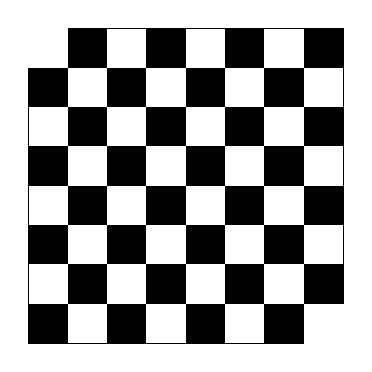
\begin{tikzpicture}[x=0.5cm,y=0.5cm]
    \foreach \x in {0,...,7} \foreach \y in {0,...,7}
    {
        \pgfmathparse{mod(\x+\y+1,2) ? "black" : "white"}
        \edef\colour{\pgfmathresult}
        \path[fill=\colour] (\x,\y) rectangle ++ (1,1);
    }
    \draw (0,0)--(7,0);
    \draw (8,1)--(8,8)--(1,8);
    \draw (0,7)--(0,0);
\end{tikzpicture}
\end{figure}

In the course notes (pages 60 -- 61),
there's a proof that it's impossible to tile this chessboard using
$2 \times 1$ dominoes.
This question considers what happens if you try to tile the chessboard
using \textit{\textbf{right triominoes}}, L-shaped tiles that look like this:

\begin{figure}[h!]
\centering
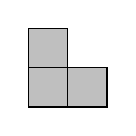
\begin{tikzpicture}[x=0.5cm,y=0.5cm]
\draw[fill=lightgray] (0,0) rectangle ++ (1,1);
\draw[fill=lightgray] (1,0) rectangle ++ (1,1);
\draw[fill=lightgray] (0,1) rectangle ++ (1,1);
\end{tikzpicture}
\end{figure}

\begin{enumerate}[label*=\roman*.,ref=\roman*]

\item Prove that it is impossible to tile an $8 \times 8$ chessboard missing
two opposite corners with right triominoes.

\begin{shaded}
Provide a proof here.
\end{shaded}

\item \textit{\textbf{Prove or disprove:}} there is a natural number $n \ge 3$ where it's possible to tile an $n \times n$ chessboard missing two corners with right triominoes.

\textit{\textcolor{blue}{ Part (ii) of this problem is another example of a prove-or-disprove type problem, and you've had plenty of practice with that from Problem Eight. So approach it the same way -- grab a sheet of scratch paper, write
out both the statement and its negation, work out what it is that you'd do if you wanted to prove each of
those statements is true, and try a lot of examples. Explore both options and see what you find! As with
part (i), drawing pictures would be a great strategy here. If you can successfully tile a board of a given size,
great! You're done. If you keep running into trouble, perhaps you can spot a pattern about why that is and
use that as the basis of a disproof. }}

\begin{shaded}
Provide a proof or disproof here.
\end{shaded}

\end{enumerate}

\section{Yablo's Paradox}

A \emph{logical paradox} is a statement that results in a contradiction
regardless of whether it's true or false.
One of the simplest paradoxes is the \emph{Liar's paradox},
which is the following:
\begin{center}
\textbf{\textit{This statement is false.}}
\end{center}
If this statement is true,
then by its own admission, it must be false -- a contradiction!
On the other hand, if the above statement is false, then the statement ``This statement is false'' is false, and therefore the
statement ``This statement is false'' is true -- a contradiction!
Since this statement results in a contradiction regardless of whether
it's true or false, its a paradox. \\

Paradoxes often arise as a result of self-reference.
In the Liar's Paradox,
the paradox arises because the statement itself directly refers to itself.
However, it's not the only paradox that can arise from self-reference.
This problem explores a paradox called \textbf{\textit{Yablo's paradox}}. \\

Consider the following collection of infinitely many statements numbered
$S_0, S_1, S_2,\dots,$ where there is a statement $S_n$ for each
natural number $n$.
These statements are ordered in a list as follows:
\begin{center}
\begin{framed}
$(S_0)$: All statements in this list after this one are false. \\
$(S_1)$: All statements in this list after this one are false. \\
$(S_2)$: All statements in this list after this one are false. \\
$\cdots$
\end{framed}
\end{center}
More generally, for each $n \in \N$,
the statement $(S_n)$ is
\begin{center}
$(S_n)$: All statements in this list after this one are false.
\end{center}
Surprisingly,
the interplay between these statements makes every statement in the list
a paradox.

\begin{enumerate}[label*=\roman*.,ref=\roman*]

\item Prove that every statement in this list is a paradox. 

\textit{\textcolor{blue}{ Some hints on this problem:
\begin{itemize}
\item We've asked you to prove a universal statement
(every element in this list is a paradox).
What is the general template for proving a universal statement?
\item Split your proof into two parts.
First, show that you get a contradiction
if any of the
statements in the list are true.
Then, show that you get a contradiction if any of the statements
in the list are false.
\item You should implicitly assume, as we've been doing in class,
that every statement is either true or false.
You don't need to worry about statements that are neither true nor false or statements that
are simultaneously true and false.
\item How do you negate a universally-quantifed statement?
\end{itemize} }}

\begin{shaded}
Provide a proof here.
\end{shaded}

\end{enumerate}

Now, consider the following modification to this list.
Instead of infinitely many statements,
suppose that there are ``only'' $10,000,000,000$ statements.
Specifically, suppose we have these statements:
\begin{center}
\begin{framed}
$(T_0)$: All statements in this list after this one are false. \\
$(T_1)$: All statements in this list after this one are false. \\
$(T_2)$: All statements in this list after this one are false. \\
$\cdots$ \\
$(T_{9,999,999,999})$: All statements in this list after this one are false.
\end{framed}
\end{center}
There's still a lot of statements here,
but not infinitely many of them.
Interestingly,
these statements are all perfectly consistent with one another and do not
result in any paradoxes.

\begin{enumerate}[resume*]

\item For each statement in the above list,
determine whether it's true or false and explain why
your choices are consistent with one another.

\begin{shaded}
\begin{answer}
Write your answer here.
\end{answer}
\end{shaded}

\end{enumerate}

Going forward, don't worry about paradoxical statements in CS103.
We won't talk about any more statements like these.
\smiley

\section*{Optional Fun Problem: The Mouse and the Cheese (1 Point Extra Credit)
\footnote{Adapted from Problem 4E of \emph{A Course in Combinatorics,
Second Edition} by van Lint and Wilson.}}

On each problem set,
we'll provide an optional fun problem for extra credit.
When we compute final grades
at the end of the quarter,
we compute the grading curve without any extra credit factored in,
then recompute
grades a second time to factor in extra credit.
This way, you're not at any disadvantage if
you decide not to work through these problems.
If you do complete the extra credit problems,
you may get a slight boost to your overall grade.
As a matter of course policy,
we don't provide any hints
on the extra credit problems -- after all,
they're supposed to be challenge problems!
However, we're happy to chat about them after the problem sets come due. \\

Suppose that you have a $3" \times 3" \times 3"$ cube of cheese
subdivided into twenty-seven $1" \times 1" \times 1"$
smaller cubes of cheese.
A mouse wants to eat the entire cube of cheese and does so as follows:
she first picks any small cube to eat first,
then moves to an adjacent small cube of cheese
(i.e. a cube that
shares a face with the cube that was just eaten)
to eat next,
then repeats this process. \\

Prove that the mouse can't eat the centermost cube of cheese last.

\begin{shaded}
Provide a proof here.
\end{shaded}

\end{document}